\documentclass[12pt]{article}
\usepackage[german]{babel}
\usepackage[parfill]{parskip}
\renewcommand{\familydefault}{\sfdefault}
\usepackage{geometry, fancyhdr}
 \geometry{
 a4paper,
 left=25mm,
 top=20mm,
 right=20mm,
 bottom=20mm
 }
\usepackage[utf8]{inputenc}
\usepackage{pdfpages}
\usepackage{amsmath,amssymb,amsfonts,amsthm,enumitem}
\newtheorem{defi}{Definition}
\newtheorem{bsp}{Beispiel}
\newtheorem{kom}{Kommentar}
\newtheorem{ass}{Eselsbrücke}
\usepackage{shadethm,multicol,float}
\usepackage{scalerel,amssymb}
\def\mcirc{\mathbin{\scalerel*{\circ}{j}}}
\def\msquare{\mathord{\scalerel*{\Box}{gX}}}
\newshadetheorem{ueb}{Übung}
\definecolor{shadethmcolor}{HTML}{EDF8FF}
\definecolor{shaderulecolor}{HTML}{45CFFF}
\setlength{\shadeboxrule}{.4pt}

\newenvironment{los}{%
     \setlength\parindent{0pt}\par\medskip\textbf{Lösung.}\quad}{%
     \hfill\tiny$\blacksquare$\par\medskip}

\usepackage{kpfonts}
\usepackage{stackengine, pstricks-add}
\usepackage{calc}
\newlength\shlength
\newcommand\vv[2][0]{\setlength\shlength{#1pt}%
  \stackengine{-5.6pt}{$#2$}{\smash{$\kern\shlength%
    \stackengine{7.55pt}{$\mathchar"017E$}%
      {\rule{\widthof{$#2$}}{.57pt}\kern.4pt}{O}{r}{F}{F}{L}\kern-\shlength$}}%
      {O}{c}{F}{T}{S}}
\usepackage{pdfpages}
\allowdisplaybreaks
\usepackage{tcolorbox}
\usepackage{geometry}

\geometry{a4paper, left=25mm, right=25mm, top=25mm, bottom=25mm}

% Header und Footer konfigurieren
\pagestyle{fancy}
\fancyhf{} % alle Standardfelder leeren

% Header (zentriert)
\fancyhead[C]{,,Europaschule'' Gymnasium Gommern}

% Footer
\fancyfoot[L]{Dr. Amar Bapic}
\fancyfoot[C]{Analysis (gAn)}
\fancyfoot[R]{\thepage}

% Linien oben und unten entfernen (optional)
\renewcommand{\headrulewidth}{0.4pt}
\renewcommand{\footrulewidth}{0.4pt}

% Farben definieren
\definecolor{myblue}{RGB}{227,242,253}
\definecolor{mygreen}{RGB}{232,245,233}

\begin{document}

\section*{Infinitesimalrechnung – Verhalten im Unendlichen}

Das Verhalten im Unendlichen beschreibt, wie sich die Funktionswerte
für sehr große positive oder sehr große negative Werte von \(x\) verhalten.

Dabei betrachtet man die Grenzwerte

\[
\lim_{x \to +\infty} f(x)
\quad \text{und} \quad
\lim_{x \to -\infty} f(x).
\]

Der Grenzwert wird auch \textit{Limes} genannt.

\begin{tcolorbox}[colback=myblue]
\textbf{Merksatz:}\\
Wenn \(x\) gegen \(+\infty\) bzw. \(-\infty\) geht und sich dabei
\(f(x)\) einem bestimmten Wert \(g\) nähert,
so sagt man, dass \(f\) den \textbf{Grenzwert} \(g\) besitzt, und schreibt:

\[
\lim_{x \to +\infty} f(x) = g
\quad \text{bzw.} \quad
\lim_{x \to -\infty} f(x) = g.
\]
\end{tcolorbox}

\begin{tcolorbox}[colback=myblue]
\textbf{Merksatz:}\\
Eine Funktion besitzt einen \textbf{uneigentlichen Grenzwert},
wenn für beliebig große bzw. kleine Werte von \(x\) der Funktionswert
beliebig groß oder beliebig klein wird.

Man schreibt:

\[
\lim_{x \to \pm\infty} f(x) = \pm\infty.
\]
\end{tcolorbox}

\section*{1. Bedeutung}

Das Verhalten im Unendlichen ist wichtig für:

\begin{itemize}
\item Bestimmung von Asymptoten
\item Skizzieren von Funktionsgraphen
\item Analyse von Wachstumsverhalten
\item Vergleich von Funktionen
\end{itemize}

\section*{2. Berechnung mit Testeinsetzung (Tabelle)}

Gegeben sei

\[
f(x)=\frac{3x^2+1}{2x^2-5}.
\]

\subsection*{Tabelle}

\begin{center}
\begin{tabular}{c|cccccccccc}
\(x\) & \dots & -10000&-1000 & -100 & -10 & 10 & 100 & 1000 &10000&\ldots \\
\hline
\(f(x)\) & \dots &1,50& 1{,}50 & 1{,}50 & 1{,}54 & 1{,}54 & 1{,}50 & 1{,}50 & 1,50&\ldots
\end{tabular}
\end{center}

\subsection*{Beobachtung}

Die Funktionswerte nähern sich sowohl für große negative als auch
für große positive Werte von \(x\) dem Wert \(1,5\).
Ist eine eindeutige Tendenz noch nicht erkennbar,
werden größere Beträge eingesetzt.

\begin{tcolorbox}[colback=mygreen]
\textbf{Ergebnis:}
\[
\lim_{x\to\pm\infty} f(x)=1,5.
\]
\end{tcolorbox}

\begin{tcolorbox}[colback=myblue]
\textbf{Hinweis:}\\
Besitzt die Funktion \(f\) einen Grenzwert \(g\), so ist die Gerade
\[y=g\] eine \textbf{waagerechte Asymptote} (eine Gerade, die sich der Graph einer Funktion immer weiter annähert, wenn man sich in die positive bzw. negative x-Richtung entfernt).
\end{tcolorbox}

\begin{figure}[H]
\centering
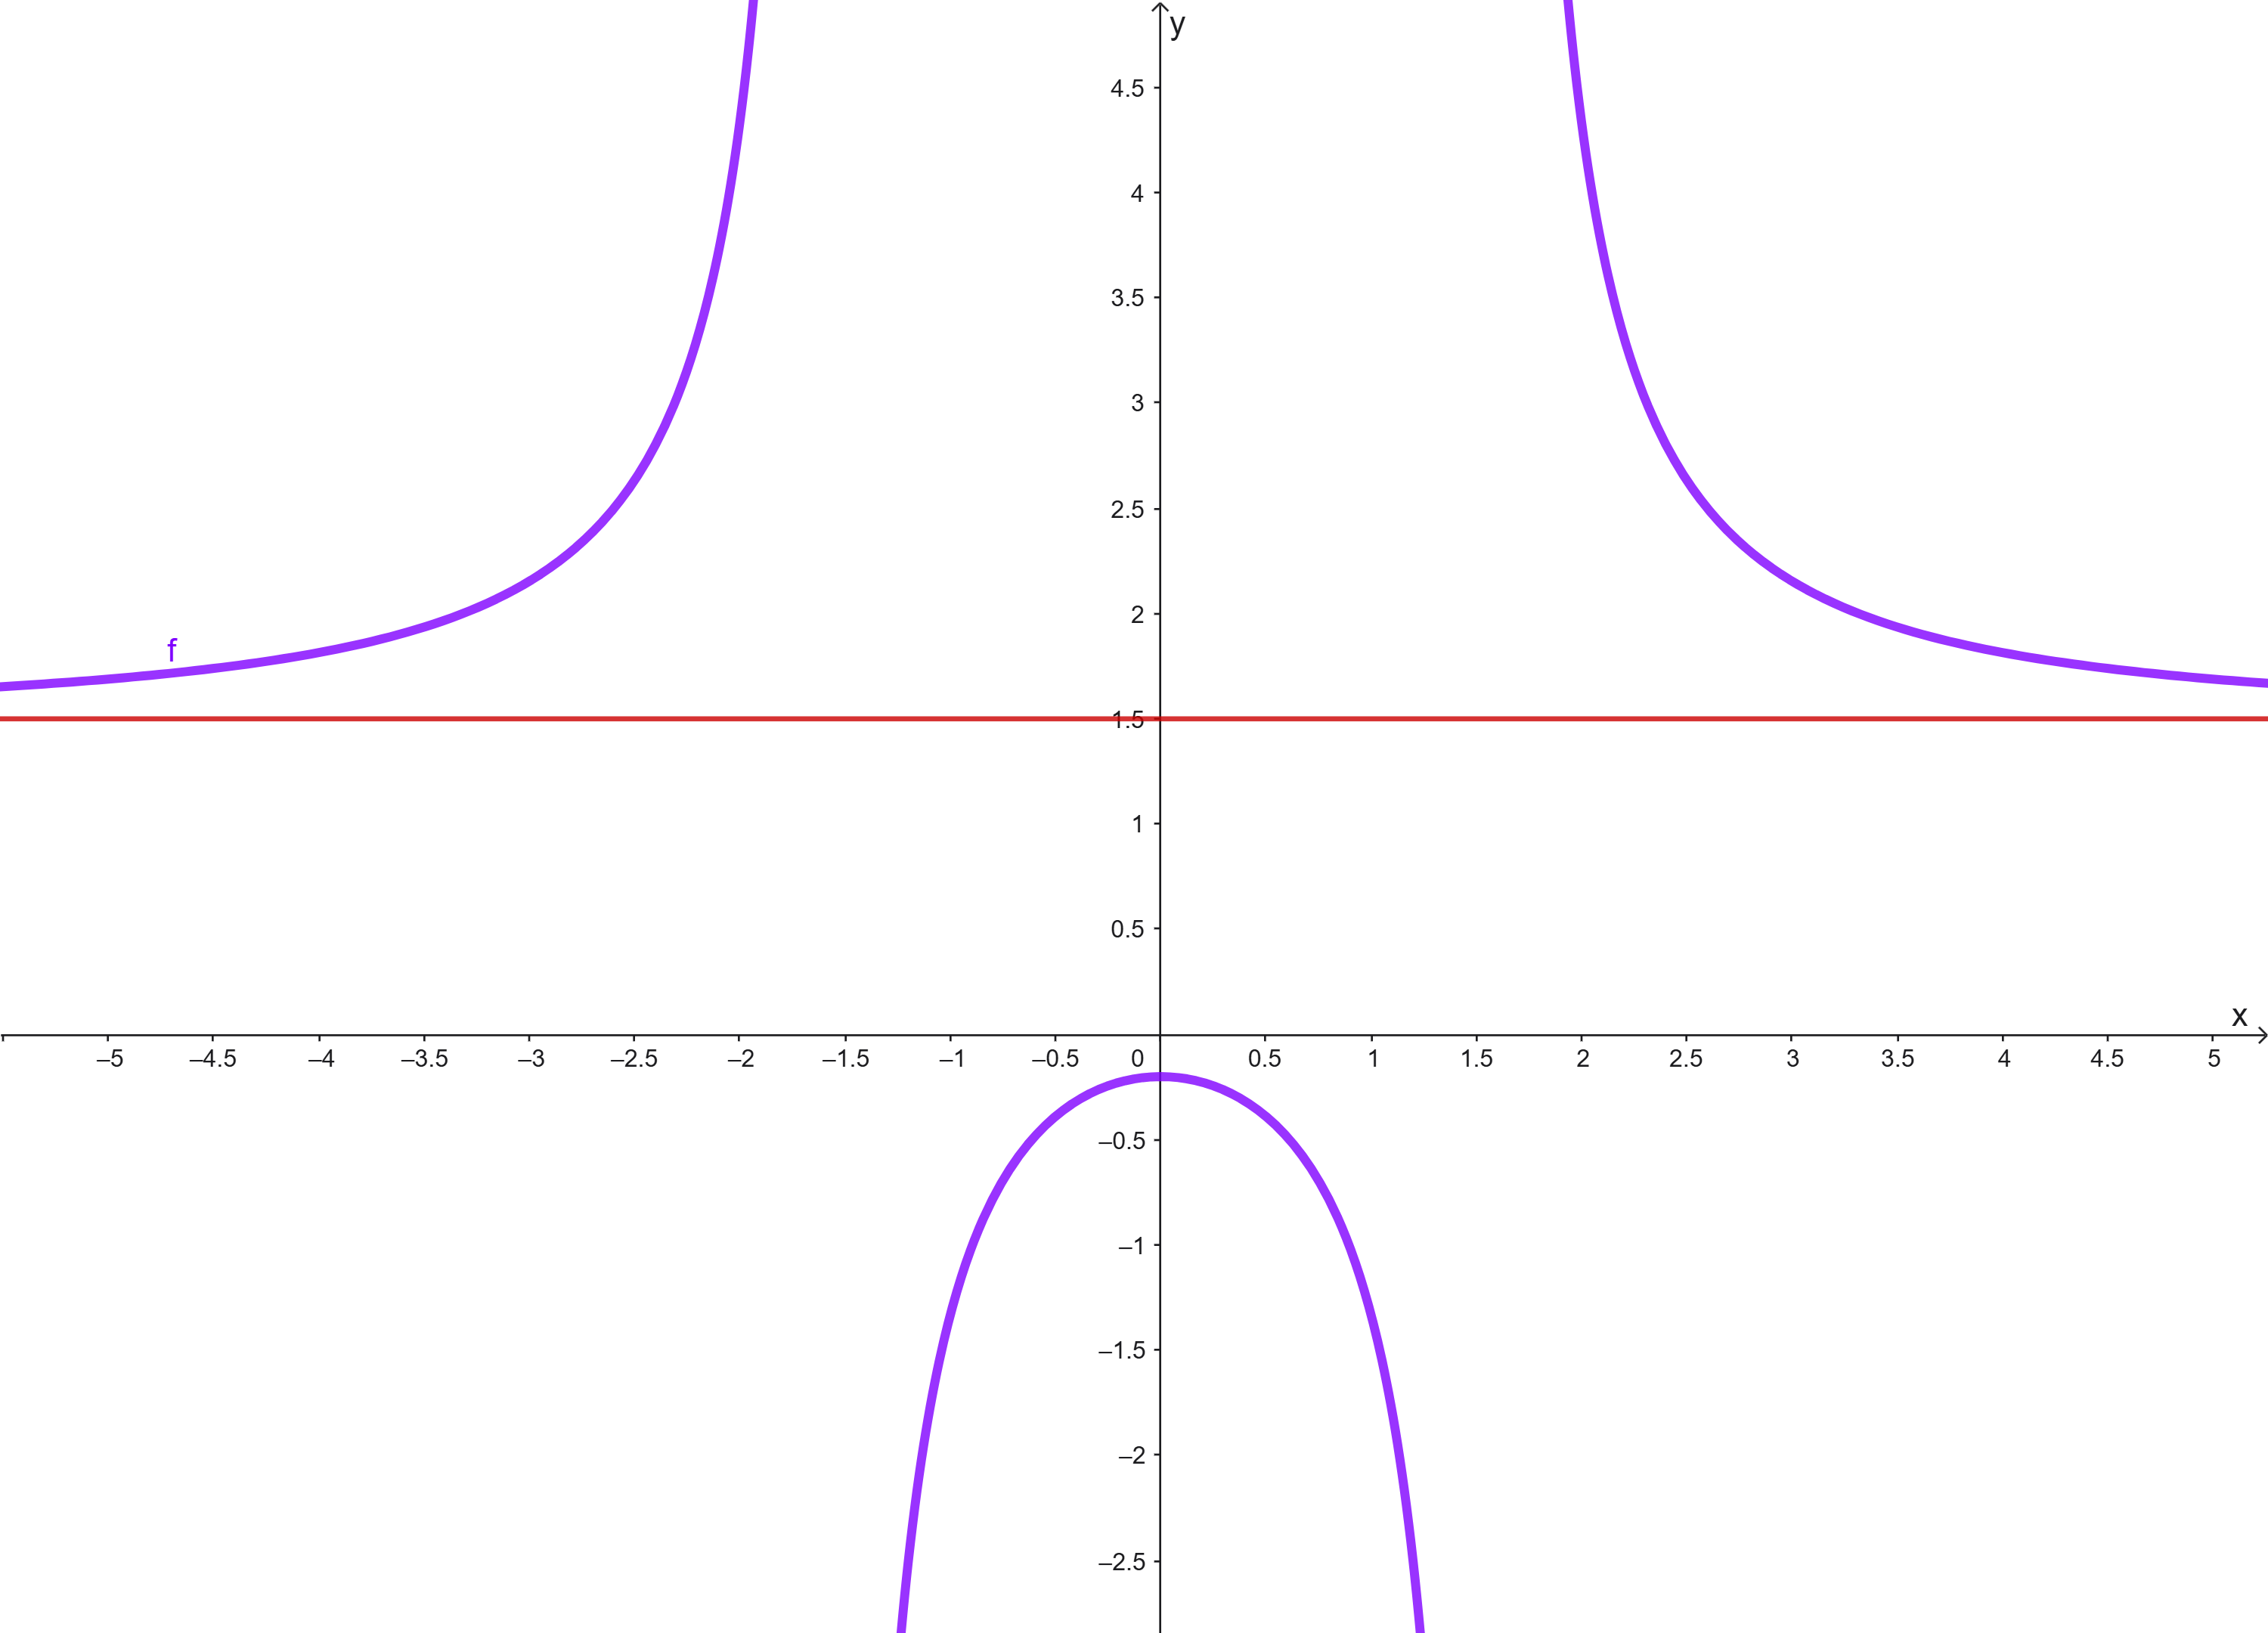
\includegraphics[width=\textwidth]{assets/images/bsp1.png}
\end{figure}

\newpage

\subsection*{Beispiel: Uneigentlicher Grenzwert (\(\pm\infty\))}

Gegeben sei \(
f(x)=x^2-3x+1.
\)

\begin{center}
\begin{tabular}{c|ccccccc}
\(x\) & \dots & -1000 & -100 & -10 & 10 & 100 & 1000 \\
\hline
\(f(x)\) & \dots & 1003001 & 10301 & 131 & 71 & 9701 & 997001
\end{tabular}
\end{center}

\begin{tcolorbox}[colback=mygreen]
\textbf{Ergebnis:}
\[
\lim_{x\to+\infty} f(x)=+\infty,
\qquad
\lim_{x\to-\infty} f(x)=+\infty.
\]
\end{tcolorbox}

\begin{figure}[H]
\centering
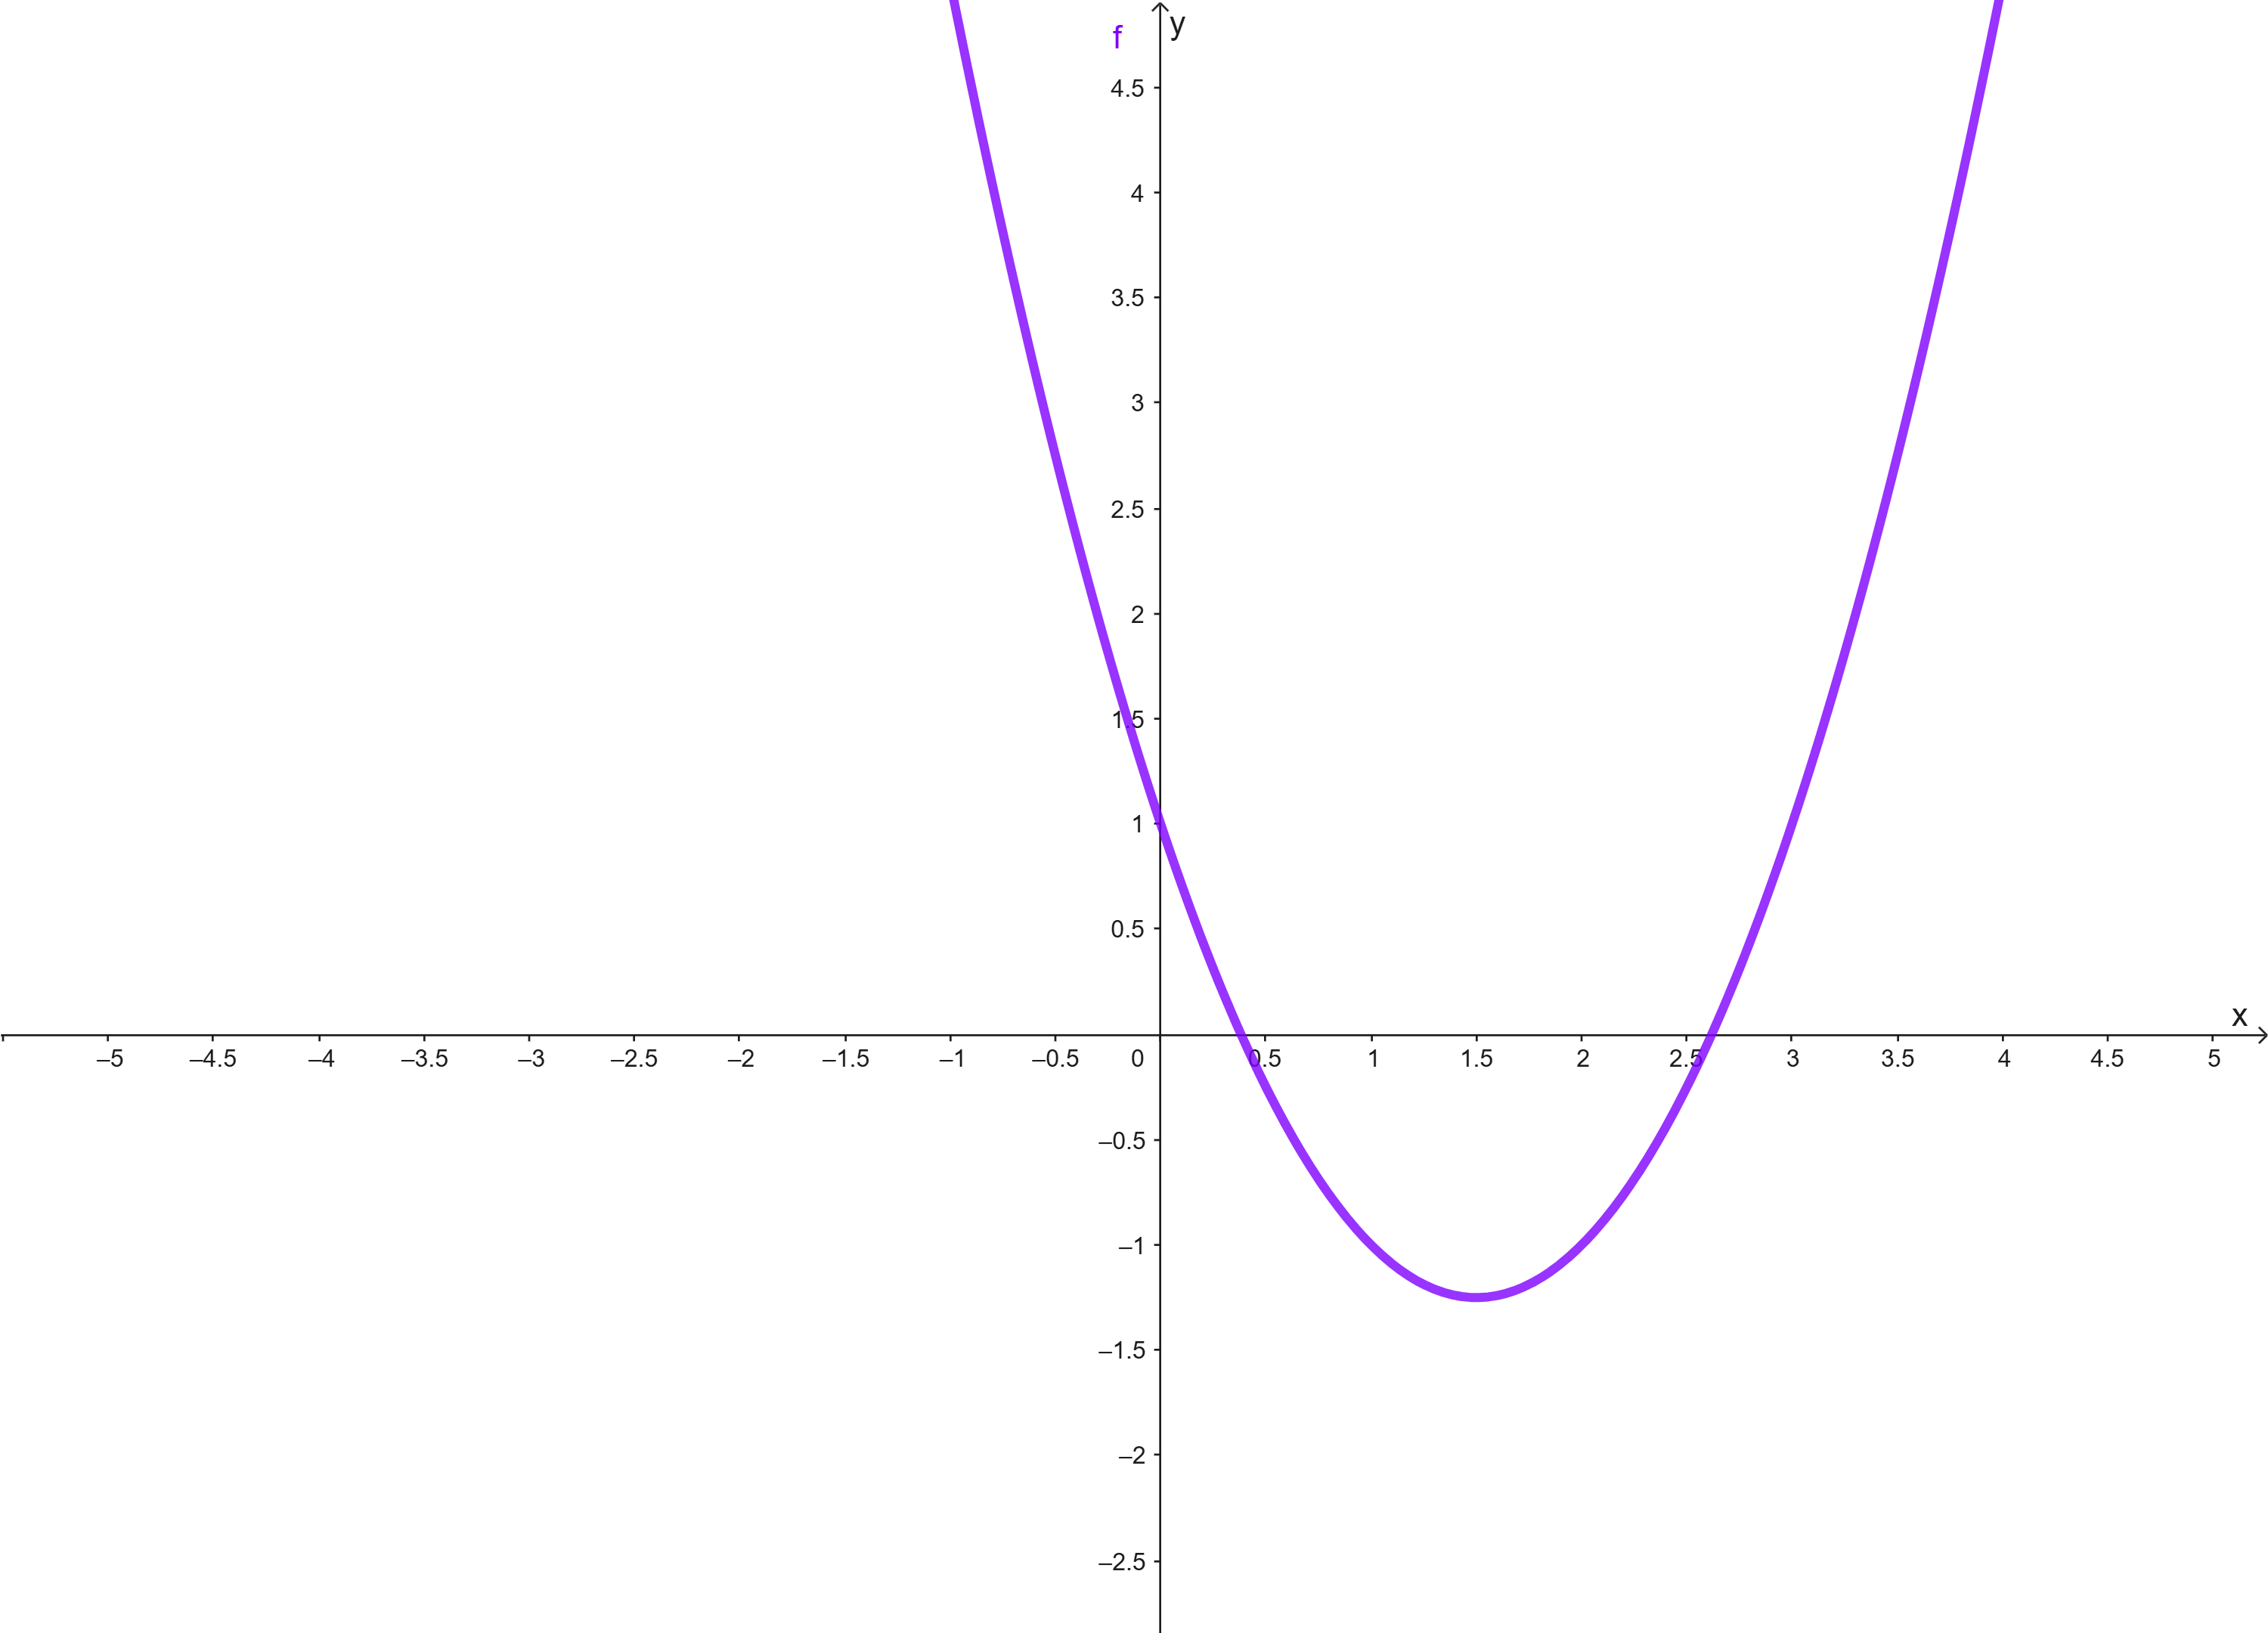
\includegraphics[width=0.4\textwidth]{assets/images/bsp2.png}
\end{figure}

\subsection*{Beispiel: Unterschiedliche Grenzwerte}

Gegeben sei

\[
f(x)=\frac{2x}{\sqrt{x^2+1}}.
\]

\begin{center}
\begin{tabular}{c|ccccccc}
\(x\) & \dots & -1000 & -100 & -10 & 10 & 100 & 1000 \\
\hline
\(f(x)\) & \dots & -2{,}00 & -2{,}00 & -1{,}99 & 1{,}99 & 2{,}00 & 2{,}00
\end{tabular}
\end{center}

\begin{tcolorbox}[colback=mygreen]
\textbf{Ergebnis:}
\[
\lim_{x\to+\infty} f(x)=2,
\qquad
\lim_{x\to-\infty} f(x)=-2.
\]

Die Funktion besitzt zwei verschiedene waagerechte Asymptoten:
\(y=2\) rechts und \(y=-2\) links.
\end{tcolorbox}

\begin{figure}[H]
\centering
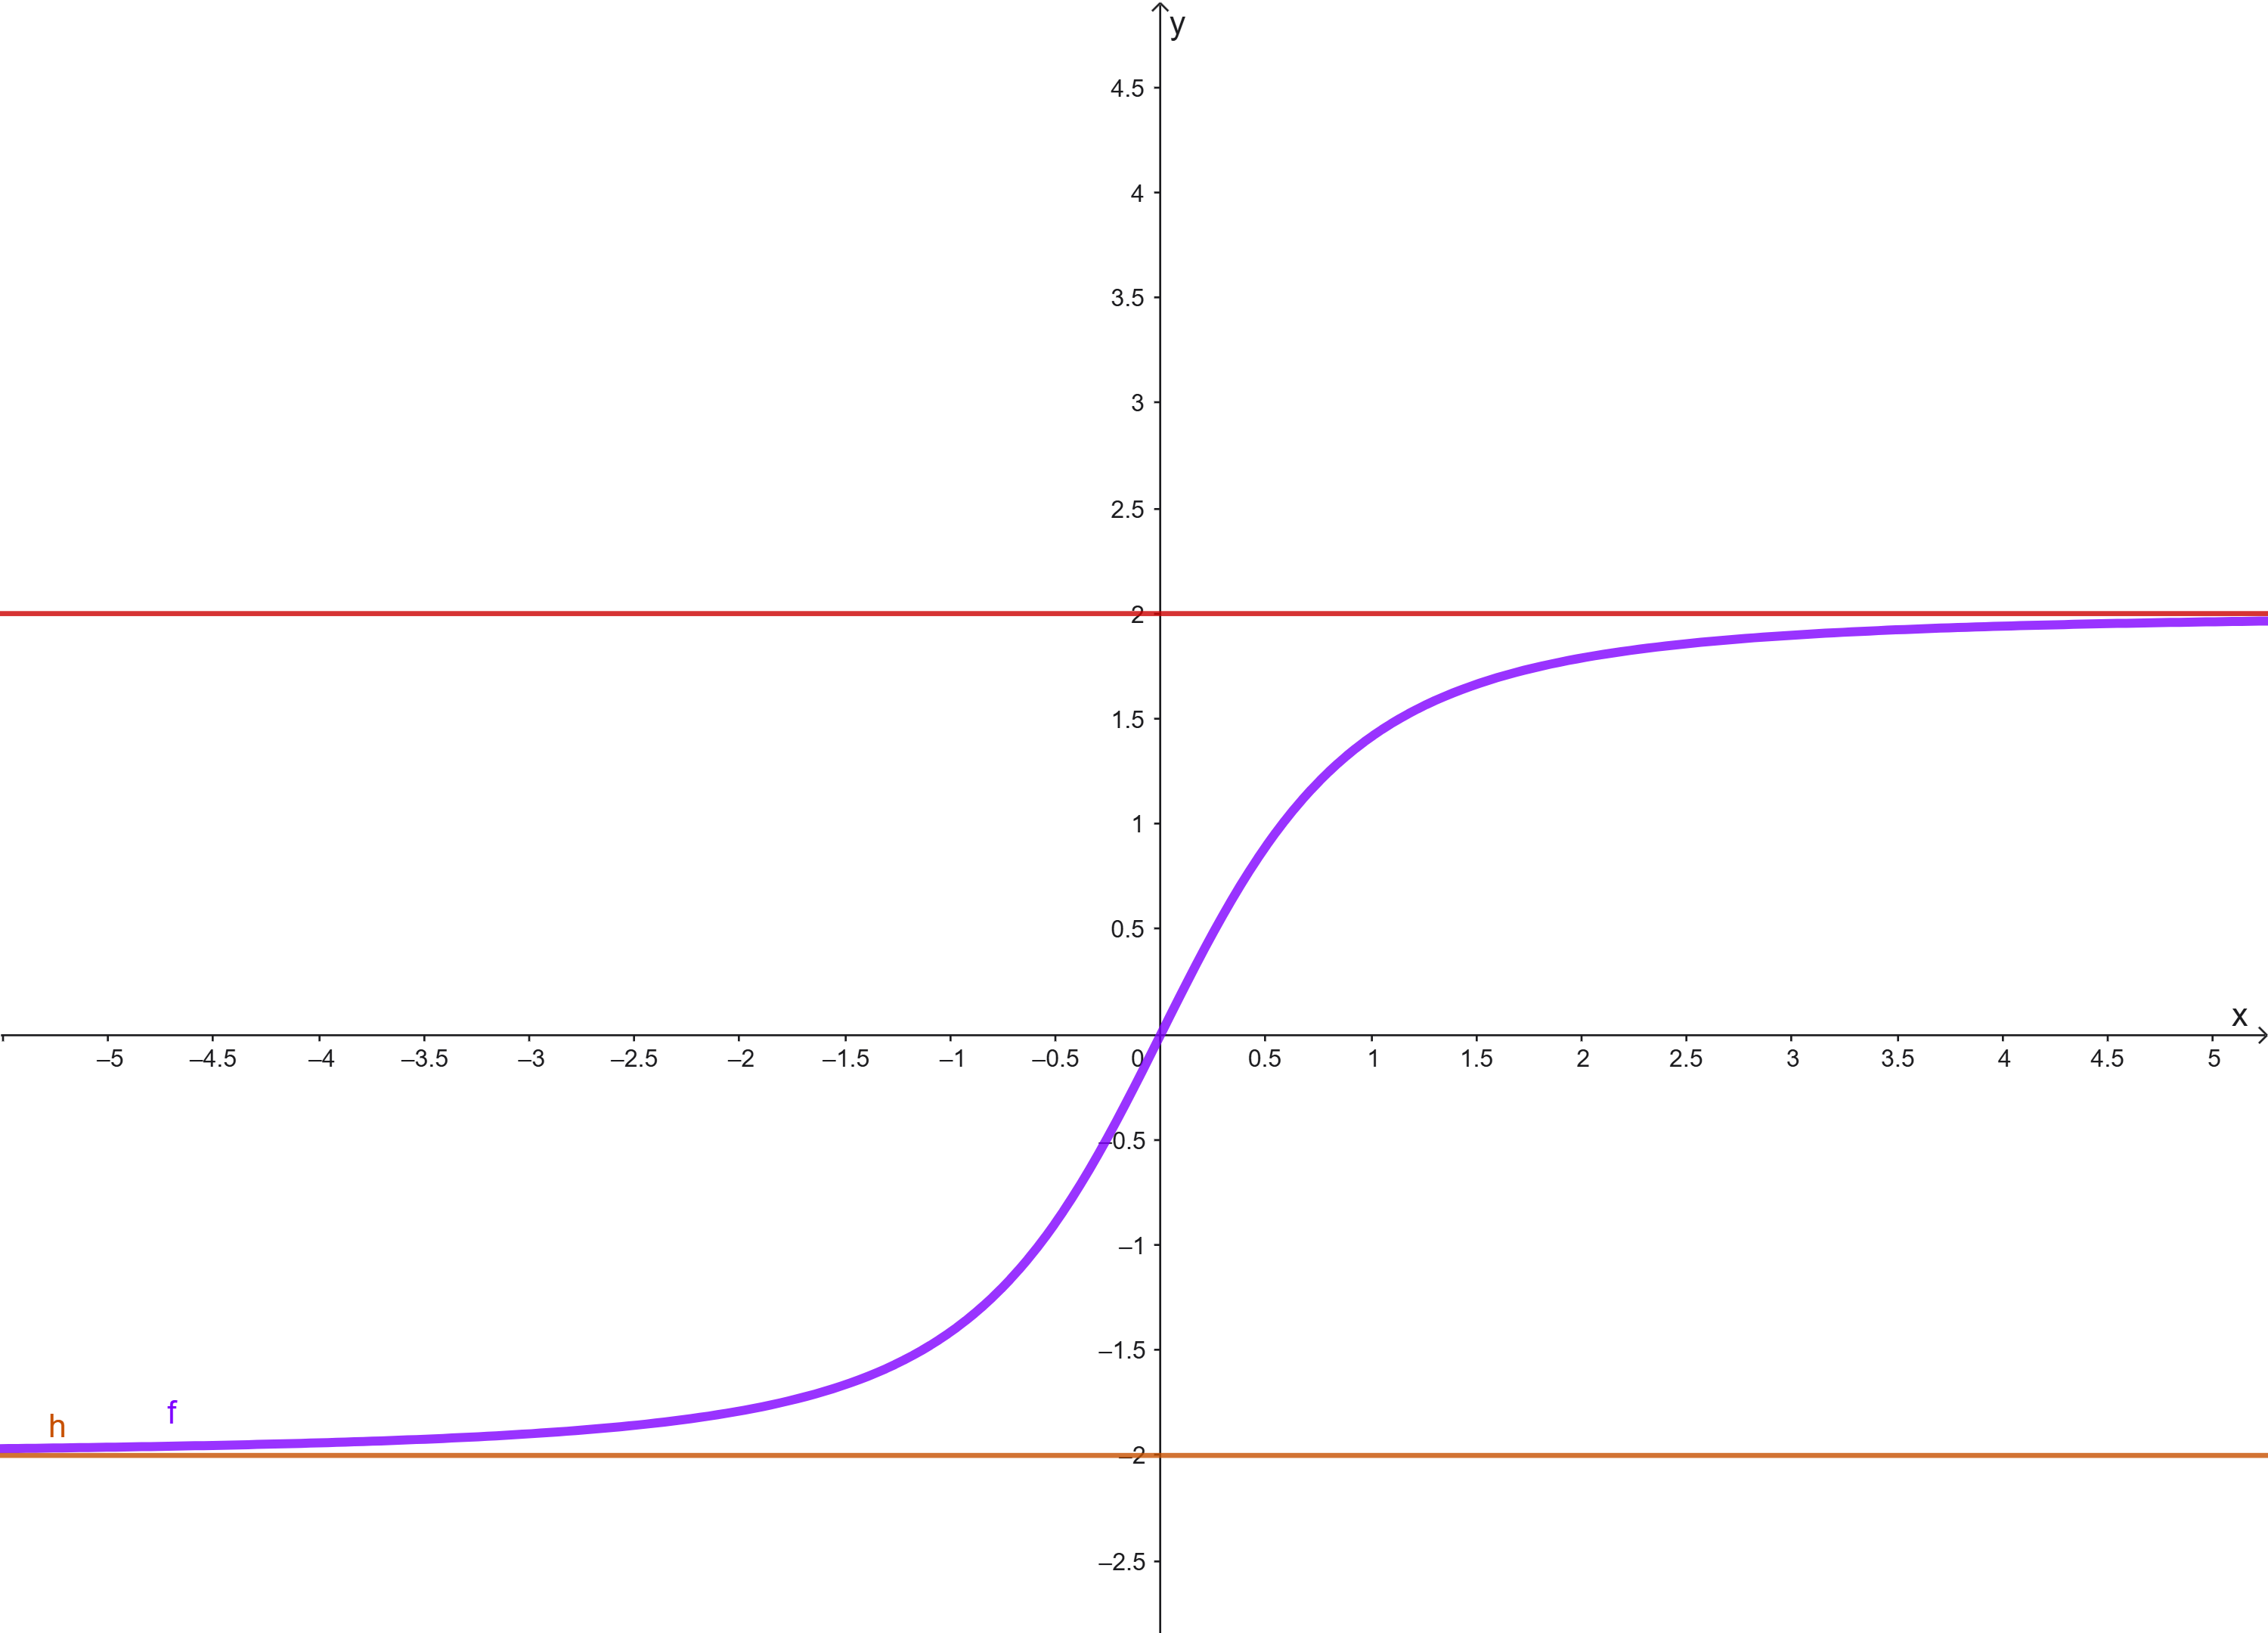
\includegraphics[width=0.5\textwidth]{assets/images/bsp3.png}
\end{figure}

\end{document}
